%!TEX TS-program = xelatex

% Шаблон документа LaTeX создан в 2018 году
% Алексеем Подчезерцевым
% В качестве исходных использованы шаблоны
% 	Данилом Фёдоровых (danil@fedorovykh.ru) 
%		https://www.writelatex.com/coursera/latex/5.2.2
%	LaTeX-шаблон для русской кандидатской диссертации и её автореферата.
%		https://github.com/AndreyAkinshin/Russian-Phd-LaTeX-Dissertation-Template

\documentclass[a4paper,14pt]{article}

%%% Работа с русским языком
\usepackage[english,russian]{babel}   %% загружает пакет многоязыковой вёрстки
\usepackage{fontspec}      %% подготавливает загрузку шрифтов Open Type, True Type и др.
\defaultfontfeatures{Ligatures={TeX},Renderer=Basic}  %% свойства шрифтов по умолчанию
\setmainfont[Ligatures={TeX,Historic}]{Times New Roman} %% задаёт основной шрифт документа
\setsansfont{Comic Sans MS}                    %% задаёт шрифт без засечек
\setmonofont{Courier New}
\usepackage{indentfirst}
\frenchspacing

\renewcommand{\epsilon}{\ensuremath{\varepsilon}}
\renewcommand{\phi}{\ensuremath{\varphi}}
\renewcommand{\kappa}{\ensuremath{\varkappa}}
\renewcommand{\le}{\ensuremath{\leqslant}}
\renewcommand{\leq}{\ensuremath{\leqslant}}
\renewcommand{\ge}{\ensuremath{\geqslant}}
\renewcommand{\geq}{\ensuremath{\geqslant}}
\renewcommand{\emptyset}{\varnothing}

%%% Дополнительная работа с математикой
\usepackage{amsmath,amsfonts,amssymb,amsthm,mathtools} % AMS
\usepackage{icomma} % "Умная" запятая: $0,2$ --- число, $0, 2$ --- перечисление

%% Номера формул
%\mathtoolsset{showonlyrefs=true} % Показывать номера только у тех формул, на которые есть \eqref{} в тексте.
%\usepackage{leqno} % Нумерация формул слева	

%% Перенос знаков в формулах (по Львовскому)
\newcommand*{\hm}[1]{#1\nobreak\discretionary{}
	{\hbox{$\mathsurround=0pt #1$}}{}}

%%% Работа с картинками
\usepackage{graphicx}  % Для вставки рисунков
\graphicspath{{images/}}  % папки с картинками
\setlength\fboxsep{3pt} % Отступ рамки \fbox{} от рисунка
\setlength\fboxrule{1pt} % Толщина линий рамки \fbox{}
\usepackage{wrapfig} % Обтекание рисунков текстом

%%% Работа с таблицами
\usepackage{array,tabularx,tabulary,booktabs} % Дополнительная работа с таблицами
\usepackage{longtable}  % Длинные таблицы
\usepackage{multirow} % Слияние строк в таблице
\usepackage{float}% http://ctan.org/pkg/float

%%% Программирование
\usepackage{etoolbox} % логические операторы


%%% Страница
\usepackage{extsizes} % Возможность сделать 14-й шрифт
\usepackage{geometry} % Простой способ задавать поля
\geometry{top=20mm}
\geometry{bottom=20mm}
\geometry{left=20mm}
\geometry{right=10mm}
%
%\usepackage{fancyhdr} % Колонтитулы
% 	\pagestyle{fancy}
%\renewcommand{\headrulewidth}{0pt}  % Толщина линейки, отчеркивающей верхний колонтитул
% 	\lfoot{Нижний левый}
% 	\rfoot{Нижний правый}
% 	\rhead{Верхний правый}
% 	\chead{Верхний в центре}
% 	\lhead{Верхний левый}
%	\cfoot{Нижний в центре} % По умолчанию здесь номер страницы

\usepackage{setspace} % Интерлиньяж
\onehalfspacing % Интерлиньяж 1.5
%\doublespacing % Интерлиньяж 2
%\singlespacing % Интерлиньяж 1

\usepackage{lastpage} % Узнать, сколько всего страниц в документе.

\usepackage{soul} % Модификаторы начертания

\usepackage{hyperref}
\usepackage[usenames,dvipsnames,svgnames,table,rgb]{xcolor}
\hypersetup{				% Гиперссылки
	unicode=true,           % русские буквы в раздела PDF
	pdftitle={Автоматизация проектных работ},   % Заголовок
	pdfauthor={Солодянкин А.А.},      % Автор
	pdfsubject={Автоматизация проектных работ},      % Тема
	pdfcreator={Солодянкин А.А.}, % Создатель
	pdfproducer={Солодянкин А.А.}, % Производитель
	pdfkeywords={Автоматизация проектных работ}, % Ключевые слова
	colorlinks=true,       	% false: ссылки в рамках; true: цветные ссылки
	linkcolor=black,          % внутренние ссылки
	citecolor=black,        % на библиографию
	filecolor=magenta,      % на файлы
	urlcolor=black           % на URL
}
\makeatletter 
\def\@biblabel#1{#1. } 
\makeatother
\usepackage{cite} % Работа с библиографией
%\usepackage[superscript]{cite} % Ссылки в верхних индексах
%\usepackage[nocompress]{cite} % 
\usepackage{csquotes} % Еще инструменты для ссылок

\usepackage{multicol} % Несколько колонок

\usepackage{tikz} % Работа с графикой
\usepackage{pgfplots}
\usepackage{pgfplotstable}

% ГОСТ заголовки
\usepackage[font=small]{caption}
%\captionsetup[table]{justification=centering, labelsep = newline} % Таблицы по правобу краю
%\captionsetup[figure]{justification=centering} % Картинки по центру


\newcommand{\tablecaption}[1]{\addtocounter{table}{1}\small \begin{flushright}\tablename \ \thetable\end{flushright}%	
\begin{center}#1\end{center}}

\newcommand{\imref}[1]{рис.~\ref{#1}}

\usepackage{multirow}
\usepackage{spreadtab}
\newcolumntype{K}[1]{@{}>{\centering\arraybackslash}p{#1cm}@{}}


\usepackage{xparse}
\usepackage{fancyvrb}

\RecustomVerbatimCommand{\VerbatimInput}{VerbatimInput}
{
	fontsize=\footnotesize    
}

\newcolumntype{?}[1]{!{\vrule width #1}}

\usepackage{tocloft}
\renewcommand{\cftsecleader}{\cftdotfill{\cftdotsep}}
\begin{document} % конец преамбулы, начало документа
\begin{titlepage}
	\begin{center}
		ПРАВИТЕЛЬСТВО РОССИЙСКОЙ ФЕДЕРАЦИИ \\
 		ФЕДЕРАЛЬНОЕ  ГОСУДАРСТВЕННОЕ АВТОНОМНОЕ \\
		ОБРАЗОВАТЕЛЬНОЕ УЧРЕЖДЕНИЕ ВЫСШЕГО ОБРАЗОВАНИЯ\\
		«НАЦИОНАЛЬНЫЙ ИССЛЕДОВАТЕЛЬСКИЙ УНИВЕРСИТЕТ\\
		«ВЫСШАЯ ШКОЛА ЭКОНОМИКИ»
	\end{center}
	
	\begin{center}
		\textbf{Московский институт электроники и математики}
		
		\textbf{Им. А.Н.Тихонова НИУ ВШЭ}
		
		\vspace{2ex}
		
		\textbf{Департамент компьютерной инженерии}
	\end{center}
	\vspace{1ex}	
	
	\vspace{1ex}
	\begin{center}
		\textbf{Практическая работа №7 \\
			<<Математические модели для решения задач размещения на печатной плате>> \\
			по курсу <<Автоматизация проектных работ>>\\
	}
	\end{center}	

	\vspace{2ex}
	\vfill
	
	\vspace{2ex}
	
	\begin{flushright}
		\textbf{Выполнил:}
		
		\vspace{2ex}
		
		Студент группы БИВ174
		
		\vspace{2ex}
		
		Солодянкин Андрей Александрович
		
		\vspace{2ex}
		
		\textbf{Проверил:}
		
		\vspace{2ex}
		
		Новиков Константин Викторович
	\end{flushright}

	\vspace{5ex}
	\begin{center}
		Москва \the\year \, г.
	\end{center}
	
\end{titlepage}
\addtocounter{page}{1}
\tableofcontents
\pagebreak

\section{Задание}

Определить динамический диапазон схем транзисторного фильтра на частоте 1 кГц, т.е. определить максимальную амплитуду входного синусоидального сигнала, при которой выходной сигнал остается без изменений.

\section{Краткие теоретические сведения}

Временная область.

Временная область удобна при изображении изменений сигнала во времени. 
Мы все знаем, что такое синусоиды. 
Каждая синусоида характеризуется тремя параметрами: амплитудой, начальной фазой и частотой. 
Одна синусоида имеет одну частоту. 
Частота -- это параметр, показывающий как часто сигнал повторяет сам себя. 
Обратным частоте является период. 
Он соответствует продолжительности, которую занимает во времени один период периодического сигнала. 
На графиках показаны две синусоиды с различными частотами и, следовательно, различными периодами.

\section{Выполнение работы}
	
Схема фильтра представлена на рис.~\ref{fig:schema}, неискаженный сигнал на рис.~\ref{fig:wave_1}.
При $V_{in} = 3.5V$ начинают появляться искажения (рис.~\ref{fig:wave_2}).
Таким образом, динамический диапазон фильтра 3.5В.

\begin{figure}[H]
	\centering
	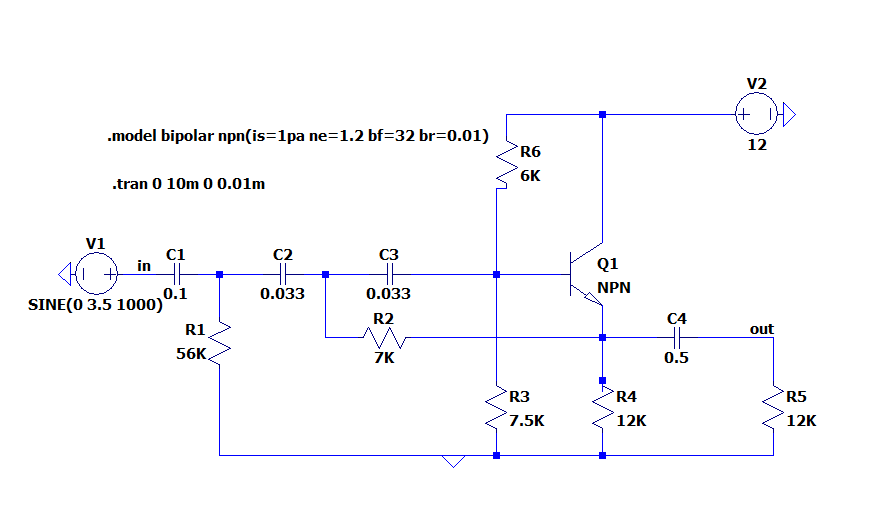
\includegraphics[width=\linewidth]{image/schema}
	\caption{Схема фильтра}
	\label{fig:schema}
\end{figure}

\begin{figure}[H]
	\centering
	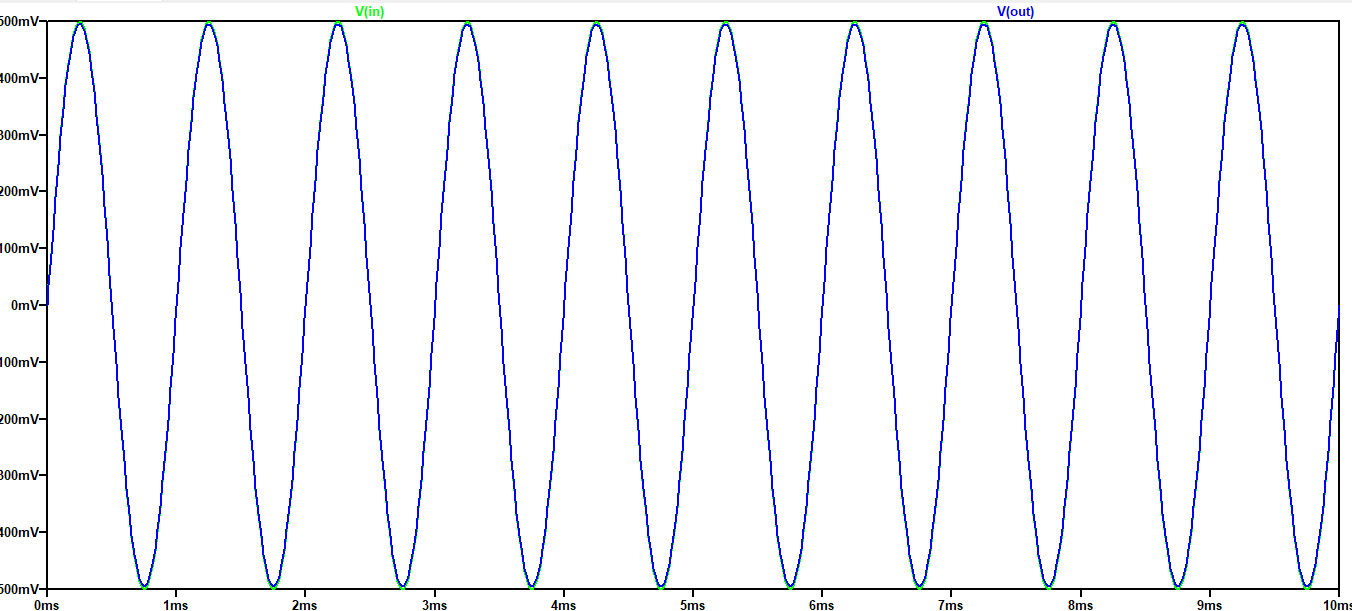
\includegraphics[width=\linewidth]{image/wave_1}
	\caption{Временная характеристика при $V_{in} = 0.5V$}
	\label{fig:wave_1}
\end{figure} 

\begin{figure}[H]
	\centering
	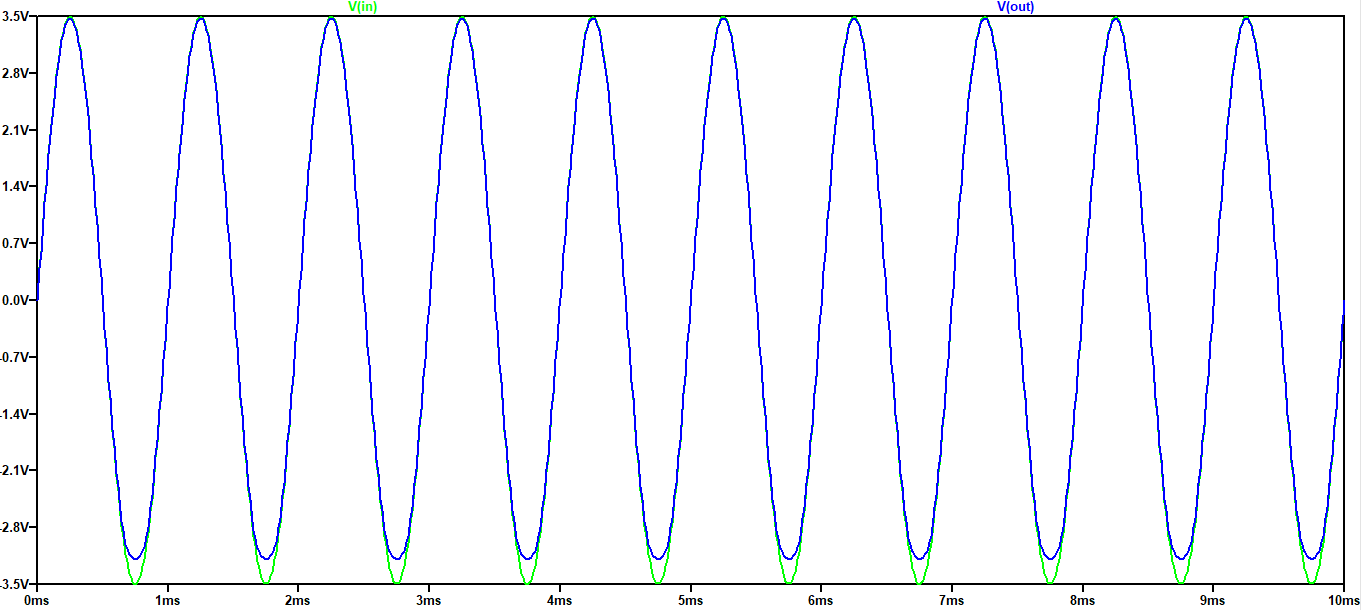
\includegraphics[width=\linewidth]{image/wave_2}
	\caption{Временная характеристика при $V_{in} = 3.5V$}
	\label{fig:wave_2}
\end{figure}
\section{Выводы по работе}

В	ходе  выполнения  работы  были  изучены  методы  математического моделирования транзисторного фильтра во временной области. Экспериментальным путем получен динамический диапазон транзисторного фильтра на частоте 1 кГц с напряжением питания 12 В, равный 3.5 В.


\section{Контрольные вопросы}

\begin{enumerate}
	\item Математическая модель схемы во временной области.
	 
	\begin{equation}
		I(V', V, t) = 0
	\end{equation}
	где $I$ - нелинейная вектор-функция, представляющая собой 
	алгебраическую сумму токов в узле;
	$V'$ - вектор производных узловых потенциалов по времени;
	$V$ - вектор узловых потенциалов;
	$t$ - время. 
	
	\item Методы решения систем дифференциальных уравнений.
	
	Существует несколько методов решения систем дифференциальных уравнений.
	Некоторые из них: метод исключения, метод характеристического уравнения (метод Эйлера), усовершенствованный метод Эйлера, метод Рунге-Кутты 4-го порядка.
\end{enumerate}

\end{document} % конец документа